\section{Experimental Study}\label{sec:expr}
To study the performance of \tool, we compare it to state-of-the-art tool \minibones~\cite{JLM15} and analysis total solving time for different groups of formulae.
We implemented \tool in C++ interfacing MINISAT 2.2 \cite{MINISAT}.The experiments were conducted on a cluster of IBM iDataPlex 2.83 GHz, each industrial formula was running with a memory limit of 4GB. Each random formula was running with a memory limit of 256 MB.

In the experiments, we separate formulae into groups. For example, if a set of formulae are generated from the application of hardware model checking, then they belong to the same group. We study the performance of \tool in 3 different groups, under different time limits. In 3600 seconds, results show that \tool saved 21\% solving time in total and performs the best in $\textit{manthey}$ group, saving 34\% of solving time. In 16000 seconds, results show that \tool solved 2 more formulae (49 formulae) than \minibones does.
We also conduct experiments on 86 groups of random formulae, \tool saved 0.4\% solving time among all random formulae. In all 86 groups, \tool performs faster than \minibones on 58 of them.

Experiments show that both \tool and \minibones are good at solving industrial formulae which have clear partitions of variables. For the solved formulae, \tool performs better than \minibones in general, especially on more complex formulae. \tool performs better on industrial formulae, which are more complex than random formulae. In the experiments of random formulae, results indicate that \tool is good at solving formula with more variables that have over 10 adjacent variables. More adjacent variables make the formula more complex. 
\subsection{Benchmark Setup}

% It's available at xxx.
We selected 72 industrial formulae and 100 crafted formulae from SAT competitions between 2002 and 2016. Results show that non of the crafted formula is solved by any tool. Therefore, instead of using crafted formulae, we generate 6600 satisfiable formulae from 86 unsatisfiable formulae, selected from Uniform-3-SAT problem. The formulae generated from the same unsatisfiable formula shared the same features and all 6600 formulae have the same variables and clauses number. We consider it fair using random formulae to test the scalability of \tool and \minibones, since both of them applied MINISAT as its SAT solver.
There are 3 groups among industrial formulae, which are $\textit{mrpp}$, $\textit{manthey}$ and $\textit{dimacs}$. And 86 groups among 6600 random formulae, separated by the original unsatisfiability formulae naturally.

\subsection{Means of Presentation}
The experiments consists of two parts, the first part shows the results in industrial formulae and the second part shows results among random formulae.
We use $\textbf{st}$ to denote the solving time and $\textbf{sc}$ to represent SAT testings number.
Comparisons of solving time among individual formula are shown as plots figures. In the figures, each line represents a tool performance of the formulae. The x-axis stands for the individual formula and the y-axis stands for the solving time of the corresponding formula.

\subsection{Experimental Results on Industrial Formulae}\label{sec:ind_expr}
Among the 72 industrial formulae, both \tool and \minibones are able to solve 34 of them in 3600 seconds (1 hour).
If more solving time is provided, \tool solved 49 formulae in 16000 seconds (almost 5 hours) while \minibones solved 47 formulae.
The details of solving time and SAT tests number comparison of each group are shown in Table \ref{tab:ind} (with 1 hour time limits). We can observe that \tool performs the best on $\textit{manthey}$ group, saved 34\% solving time, with 17\% saving on SAT testings. In total, \tool saved 21\% solving time and 16\% SAT testings. \tool saved 11\% solving time and 14\% SAT testings in $\textit{mrpp}$ group, while saving 2\% time and 0.1\% SAT testings in $\textit{dimacs}$ group. It proves the observation in \cite{JLM15} from experiment concepts that less SAT testing will lead to a faster solving.
Figure \ref{fig:ind} shows the solving time of all 34 industrial formulae, there are only 3 formulae that \minibones outperforms \tool.

When we take a look at the formulae in $\textit{manthey}$ group that \tool performs the best, we find that they all have a star-like adjacent structure as shown in Figure \ref{fig:cs}(a). It means that the variables is separate into different partitions, different variables from different partitions only appears in a few clauses at the same time. Each branch in the graph stands for a partition.



\begin{table}[t]
\centering
\begin{tabular}{ccccccc}
\toprule
 Benchmark &$\textbf{st}$ of \tool(s) &$\textbf{st}$ of \minibones (s) & $\textbf{st}$ Difference &$\textbf{sc}$ of \tool &$\textbf{sc}$ of \minibones \\
\midrule
mrpp & 6112 & 6900 & \textbf{11\%} & 19541 & 22839 \\
manthey & 4845 & 7363 & \textbf{34\%} & 49356 & 59562 \\
dimacs & 1339 & 1369 & \textbf{2\%} & 2018 & 2022 \\
total & 12296 & 15632 & \textbf{21\%} & 70915 & 84423 \\
\bottomrule
\end{tabular}
\caption{Solving Time and SAT Tests Number Comparison on Industrial Formulae}
\label{tab:ind}
\end{table}

\begin{figure}
    \centering
    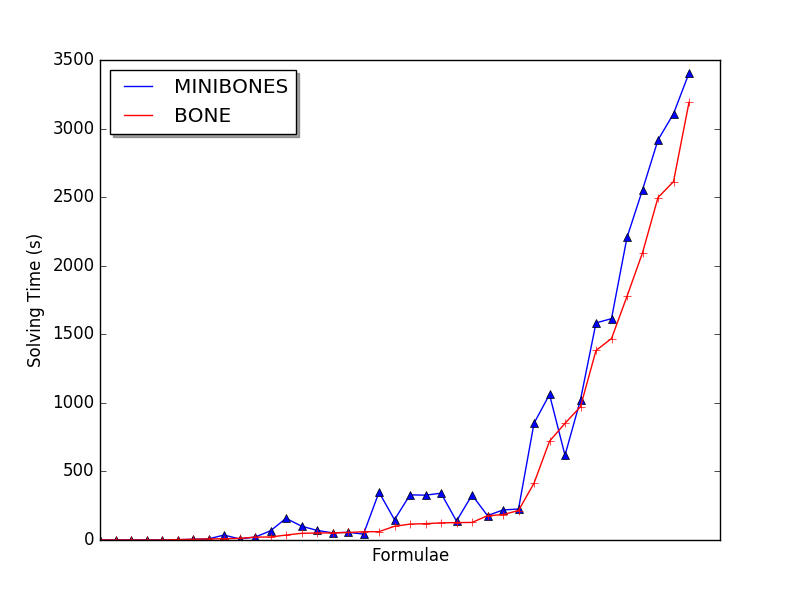
\includegraphics[scale=0.5]{ind.png}
   \caption{Solving Time Comparison on Industrial Formulae}
   \label{fig:ind}
\end{figure}

Figure \ref{fig:cs}(b) is the adjacent structure of formulae that can't be solved in 16000 seconds using both tools. It's obvious that there is no clear partition among the variables.

\begin{figure}[t]
\centering
\subfloat[Formulae with clear variables partition]{

\centering
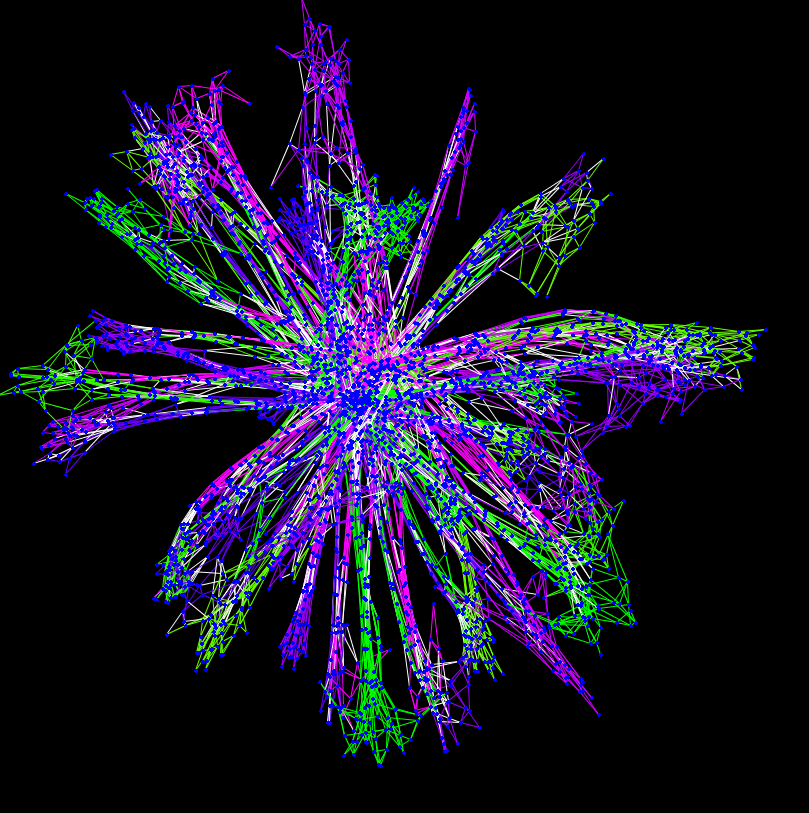
\includegraphics[width=.5\linewidth-0.45mm]{star.png}
}
\subfloat[Formulae with a tightly co-related variables]{
\centering
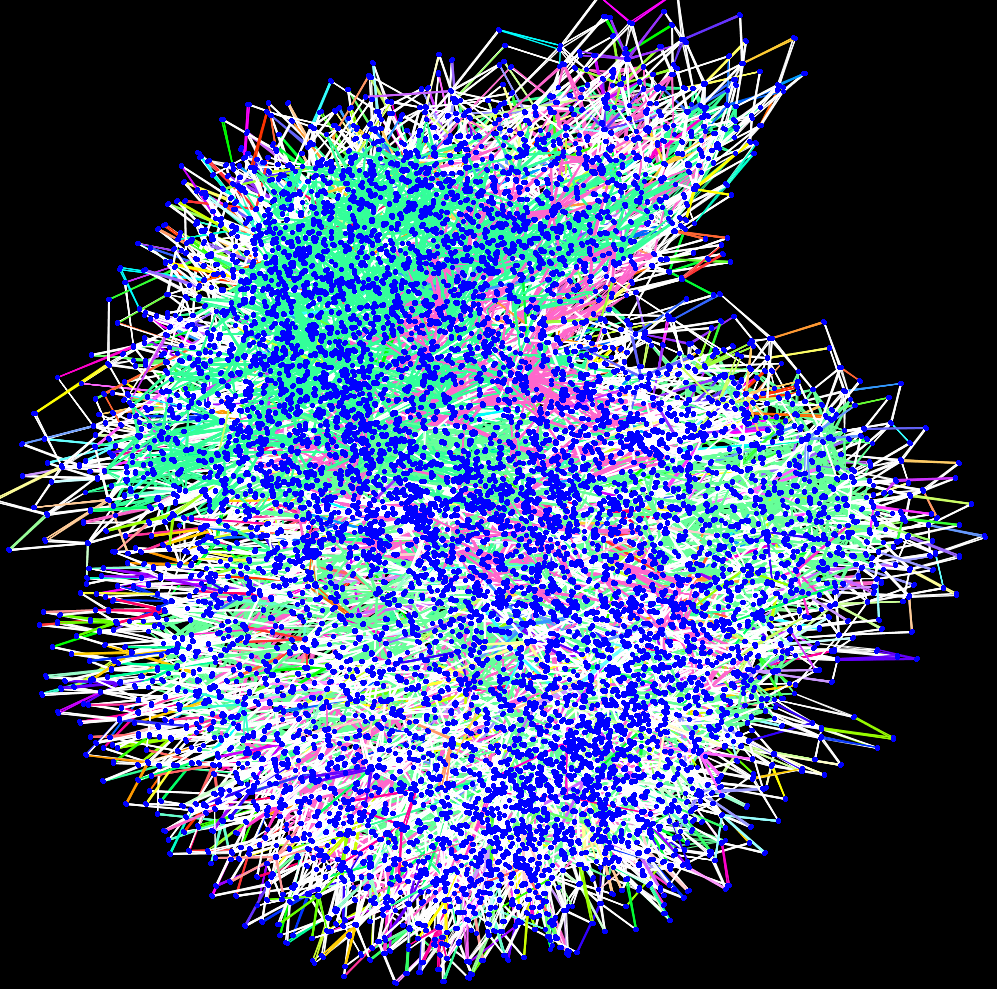
\includegraphics[width=.5\linewidth-0.45mm]{ball.png}
}
\caption{Adjacent structures}
\begin{minipage}[t]{0.9\textwidth} \small
\textit{(Figure (a) shows the star-like adjacent structure, indicates that variables separate into individual partitions, both \tool and \minibones are able to solve these formulae in 3600 seconds, \tool saved 34\% solving time in total. \\
Figure (b) shows the adjacent structure with a core and no branches, indicates that variables are tightly co-related in the formula. These formulae are more complex than the formula in \ref{fig:cs}(a), \tool solved 2 more formulae than \minibones among these formulae, within 16000 seconds)}
\end{minipage}

\label{fig:cs}
\end{figure}

For industrial formulae, \tool performs better than \minibones in general. We also found that the performance of \tool and \minibones are related to the adjacent structure of the given formula. A formula with clear partitions of variables tend to performs better on both \tool and \minibones.
To analysis the relations between formula structure and the performance of both tools, we designed and implemented experiments with 86 groups of generated formulae, consists of 6600 formulae in total. Every formula shares the same structure feature with other formula in the same group. All formulae shared the same number of variables and clauses.

\subsection{Results for Random Formulae}
Among all the 6600 random formulae, both \tool and \minibones are able to solve them within 50 seconds. Table \ref{tab:mcs_all} shows the total solving time and total SAT testings number of \tool and \minibones. 0.4\% solving time and 0.1\% SAT testings are saved by \tool.

\begin{table}[t]
\centering
\begin{tabular}{ccc}
\toprule
  &$\textbf{Solving Time}$ & $\textbf{SAT Testings Number}$ \\
\midrule
\tool & 50184 & 1508723  \\
\minibones & 50414 & 1532372 \\

\bottomrule
\end{tabular}
\caption{Solving Time and SAT Tests Number Comparison on Random Formulae}
\label{tab:mcs_all}
\end{table}

We separate the formulae into 86 groups according to the original unsatisfiable formula. \tool needs less solving time among 58 of them. Inherited from the industrial experiment, we consider the adjacent structures of different groups. Among all the 6600 generated formulae, \tool performs better for most of the case if there are more than 210 variables that have more than 10 adjacent variables. We refer variables with more than 10 adjacent variables as $\textit{active variables}$ since they appears in many clauses. It's obvious that with more active variables, the formula is more complex. We randomly select 10 formulae groups and demonstrate the average active variables number and total solving time of both tools in Table \ref{tab:mcs}. We can observe that most of the formulae performs better on \tool have more than 210 active variables.

\begin{table}[t]
\centering
\begin{tabular}{ccccc}
\toprule
Active Variables Number & $\textbf{st}$ of \tool(s) & $\textbf{st}$ of \minibones(s) & $\textbf{st}$ Difference\\
\midrule
203 & 354 & 346 & -2\% \\
208 & 614 & 574 & -6\% \\
215 & 346 & 400 & \textbf{13\%} \\
211 & 854 & 903 & \textbf{5\%} \\
215 & 365 & 381 & \textbf{4\%} \\
201 & 475 & 469 & -2\% \\
216 & 626 & 669 & \textbf{6\%} \\
204 & 643 & 592 & -7\% \\
208 & 389 & 424 & \textbf{8\%} \\
214 & 580 & 616 & \textbf{6\%} \\

\bottomrule
\end{tabular}
\caption{Active Variables Number and Solving Time of 10 Selected Random Formuale}
\label{tab:mcs}
\end{table}

\subsection{Result analysis}
Iterative SAT testings, which will hold the assignment of a literal $l$ using assumptions, take the major part of solving time in \tool. Different solving trees will be generated when choosing different $l$. The SAT testing will be faster if a SAT solving tree is able to find conflicts earlier. Conflicts will be found earlier if the chosen literal $l$ is a backbone literal and mainly appears in a small part of the clauses in the formula, due to the reducing of searching clauses. Therefore, given a formula $\Phi$ in $\textit{manthey}$ group, iterative SAT testing of a backbone literal $l\in\BL(\Phi)$ will be faster since $\Phi$ has a clear partitions of variables and each backbone literal mainly appears in a subset of $\cls(\Phi)$. In this way, computing $\BLap(\Phi)$ in \tool performs better on formulae in $\textit{manthey}$ group. There is no big difference of $\NBLap(\Phi)$ performance among groups since the computing time that $\NBLap(\Phi)$ is only related to the numbers of clauses and variables of the formula.
On the other hand, if the structures of random formulae are too simple (less than 210 variables have over 10 adjacent variables), \tool are compatible with \minibones since iterative SAT testings using both backbone and non-backbone are fast.

